\documentclass[12pt,a4paper]{article}

\usepackage{amsfonts}
\usepackage[centertags]{amsmath}
\usepackage{amsthm}
\usepackage{amssymb}

\usepackage[utf8]{inputenc}
\usepackage[french]{babel}

\usepackage{graphicx}

\leftmargin=0pt \topmargin=0pt \headheight=0in \headsep=0in \oddsidemargin=0pt \textwidth=6.5in
\textheight=8.5in


% Schriftabk¸rzungen

\newcommand{\eps}{\varepsilon}
\renewcommand{\phi}{\varphi}
\newcommand{\Sl}{\ell}    % schÀÜnes l
\newcommand{\ve}{\varepsilon}  %Epsilon

\newcommand{\BA}{{\mathbb{A}}}
\newcommand{\BB}{{\mathbb{B}}}
\newcommand{\BC}{{\mathbb{C}}}
\newcommand{\BD}{{\mathbb{D}}}
\newcommand{\BE}{{\mathbb{E}}}
\newcommand{\BF}{{\mathbb{F}}}
\newcommand{\BG}{{\mathbb{G}}}
\newcommand{\BH}{{\mathbb{H}}}
\newcommand{\BI}{{\mathbb{I}}}
\newcommand{\BJ}{{\mathbb{J}}}
\newcommand{\BK}{{\mathbb{K}}}
\newcommand{\BL}{{\mathbb{L}}}
\newcommand{\BM}{{\mathbb{M}}}
\newcommand{\BN}{{\mathbb{N}}}
\newcommand{\BO}{{\mathbb{O}}}
\newcommand{\BP}{{\mathbb{P}}}
\newcommand{\BQ}{{\mathbb{Q}}}
\newcommand{\BR}{{\mathbb{R}}}
\newcommand{\BS}{{\mathbb{S}}}
\newcommand{\BT}{{\mathbb{T}}}
\newcommand{\BU}{{\mathbb{U}}}
\newcommand{\BV}{{\mathbb{V}}}
\newcommand{\BW}{{\mathbb{W}}}
\newcommand{\BX}{{\mathbb{X}}}
\newcommand{\BY}{{\mathbb{Y}}}
\newcommand{\BZ}{{\mathbb{Z}}}

\newcommand{\Fa}{{\mathfrak{a}}}
\newcommand{\Fb}{{\mathfrak{b}}}
\newcommand{\Fc}{{\mathfrak{c}}}
\newcommand{\Fd}{{\mathfrak{d}}}
\newcommand{\Fe}{{\mathfrak{e}}}
\newcommand{\Ff}{{\mathfrak{f}}}
\newcommand{\Fg}{{\mathfrak{g}}}
\newcommand{\Fh}{{\mathfrak{h}}}
\newcommand{\Fi}{{\mathfrak{i}}}
\newcommand{\Fj}{{\mathfrak{j}}}
\newcommand{\Fk}{{\mathfrak{k}}}
\newcommand{\Fl}{{\mathfrak{l}}}
\newcommand{\Fm}{{\mathfrak{m}}}
\newcommand{\Fn}{{\mathfrak{n}}}
\newcommand{\Fo}{{\mathfrak{o}}}
\newcommand{\Fp}{{\mathfrak{p}}}
\newcommand{\Fq}{{\mathfrak{q}}}
\newcommand{\Fr}{{\mathfrak{r}}}
\newcommand{\Fs}{{\mathfrak{s}}}
\newcommand{\Ft}{{\mathfrak{t}}}
\newcommand{\Fu}{{\mathfrak{u}}}
\newcommand{\Fv}{{\mathfrak{v}}}
\newcommand{\Fw}{{\mathfrak{w}}}
\newcommand{\Fx}{{\mathfrak{x}}}
\newcommand{\Fy}{{\mathfrak{y}}}
\newcommand{\Fz}{{\mathfrak{z}}}

\newcommand{\FA}{{\mathfrak{A}}}
\newcommand{\FB}{{\mathfrak{B}}}
\newcommand{\FC}{{\mathfrak{C}}}
\newcommand{\FD}{{\mathfrak{D}}}
\newcommand{\FE}{{\mathfrak{E}}}
\newcommand{\FF}{{\mathfrak{F}}}
\newcommand{\FG}{{\mathfrak{G}}}
\newcommand{\FH}{{\mathfrak{H}}}
\newcommand{\FI}{{\mathfrak{I}}}
\newcommand{\FJ}{{\mathfrak{J}}}
\newcommand{\FK}{{\mathfrak{K}}}
\newcommand{\FL}{{\mathfrak{L}}}
\newcommand{\FM}{{\mathfrak{M}}}
\newcommand{\FN}{{\mathfrak{N}}}
\newcommand{\FO}{{\mathfrak{O}}}
\newcommand{\FP}{{\mathfrak{P}}}
\newcommand{\FQ}{{\mathfrak{Q}}}
\newcommand{\FR}{{\mathfrak{R}}}
\newcommand{\FS}{{\mathfrak{S}}}
\newcommand{\FT}{{\mathfrak{T}}}
\newcommand{\FU}{{\mathfrak{U}}}
\newcommand{\FV}{{\mathfrak{V}}}
\newcommand{\FW}{{\mathfrak{W}}}
\newcommand{\FX}{{\mathfrak{X}}}
\newcommand{\FY}{{\mathfrak{Y}}}
\newcommand{\FZ}{{\mathfrak{Z}}}

\newcommand{\CA}{{\cal A}}
\newcommand{\CB}{{\cal B}}
\newcommand{\CC}{{\cal C}}
\newcommand{\CD}{{\cal D}}
\newcommand{\CE}{{\cal E}}
\newcommand{\CF}{{\cal F}}
\newcommand{\CG}{{\cal G}}
\newcommand{\CH}{{\cal H}}
\newcommand{\CI}{{\cal I}}
\newcommand{\CJ}{{\cal J}}
\newcommand{\CK}{{\cal K}}
\newcommand{\CL}{{\cal L}}
\newcommand{\CM}{{\cal M}}
\newcommand{\CN}{{\cal N}}
\newcommand{\CO}{{\cal O}}
\newcommand{\CP}{{\cal P}}
\newcommand{\CQ}{{\cal Q}}
\newcommand{\CR}{{\cal R}}
\newcommand{\CS}{{\cal S}}
\newcommand{\CT}{{\cal T}}
\newcommand{\CU}{{\cal U}}
\newcommand{\CV}{{\cal V}}
\newcommand{\CW}{{\cal W}}
\newcommand{\CX}{{\cal X}}
\newcommand{\CY}{{\cal Y}}
\newcommand{\CZ}{{\cal Z}}

% Theorem Stil

\theoremstyle{plain}
\newtheorem{lem}{Lemma}
\newtheorem{Satz}[lem]{Satz}

\theoremstyle{definition}
\newtheorem{defn}{Definition}[section]

\theoremstyle{remark}
\newtheorem{bem}{Bemerkung}    %[section]



\newcommand{\card}{\mathop{\rm card}\nolimits}
\newcommand{\Sets}{((Sets))}
\newcommand{\id}{{\rm id}}
\newcommand{\supp}{\mathop{\rm Supp}\nolimits}

\newcommand{\ord}{\mathop{\rm ord}\nolimits}
\renewcommand{\mod}{\mathop{\rm mod}\nolimits}
\newcommand{\sign}{\mathop{\rm sign}\nolimits}
\newcommand{\ggT}{\mathop{\rm ggT}\nolimits}
\newcommand{\kgV}{\mathop{\rm kgV}\nolimits}
\renewcommand{\div}{\, | \,}
\newcommand{\notdiv}{\mathopen{\mathchoice
             {\not{|}\,}
             {\not{|}\,}
             {\!\not{\:|}}
             {\not{|}}
             }}

\newcommand{\im}{\mathop{{\rm Im}}\nolimits}
\newcommand{\coim}{\mathop{{\rm coim}}\nolimits}
\newcommand{\coker}{\mathop{\rm Coker}\nolimits}
\renewcommand{\ker}{\mathop{\rm Ker}\nolimits}

\newcommand{\pRang}{\mathop{p{\rm -Rang}}\nolimits}
\newcommand{\End}{\mathop{\rm End}\nolimits}
\newcommand{\Hom}{\mathop{\rm Hom}\nolimits}
\newcommand{\Isom}{\mathop{\rm Isom}\nolimits}
\newcommand{\Tor}{\mathop{\rm Tor}\nolimits}
\newcommand{\Aut}{\mathop{\rm Aut}\nolimits}

\newcommand{\adj}{\mathop{\rm adj}\nolimits}

\newcommand{\Norm}{\mathop{\rm Norm}\nolimits}
\newcommand{\Gal}{\mathop{\rm Gal}\nolimits}
\newcommand{\Frob}{{\rm Frob}}

\newcommand{\disc}{\mathop{\rm disc}\nolimits}

\renewcommand{\Re}{\mathop{\rm Re}\nolimits}
\renewcommand{\Im}{\mathop{\rm Im}\nolimits}

\newcommand{\Log}{\mathop{\rm Log}\nolimits}
\newcommand{\Res}{\mathop{\rm Res}\nolimits}
\newcommand{\Bild}{\mathop{\rm Bild}\nolimits}

\renewcommand{\binom}[2]{\left({#1}\atop{#2}\right)}
\newcommand{\eck}[1]{\langle #1 \rangle}
\newcommand{\wi}{\hspace{1pt} < \hspace{-6pt} ) \hspace{2pt}}


\begin{document}

\pagestyle{empty}

\begin{center}
{\huge Lösungen zur Vorrundenprüfung 2012} \\
\end{center}
\vspace{8mm}

Zuerst einige Bemerkungen zum Punkteschema. Eine vollständige und korrekte Lösung einer Aufgabe ist jeweils 7 Punkte wert. Für Komplette Lösungen mit kleineren Fehlern oder Ungenauigkeiten, die aber keinen wesentlichen Einfluss auf die Richtigkeit der dargestellten Lösung haben, geben wir 6 Punkte. Bei unvollständigen Lösungen wird der Fortschritt und der Erkenntnissgewinn bewertet (Teilpunkte). Oft gibt es mehrere Lösungen für ein Problem. Versucht jemand zum Beispiel eine Aufgabe auf zwei verschiedenen Wegen zu lösen, erreicht auf dem ersten Weg 3 Punkte, auf dem zweiten 2 Punkte, dann wird seine Punktzahl nicht 5, sondern 3 sein. Punkte, die auf verschiedenen Wegen erreicht werden, sind also \emph{nicht} kumulierbar. Die unten angegebenen Bewertungsschemata sind nur Orientierungshilfe. Gibt jemand eine alternative Lösung, dann werden wir versuchen, die Punktzahl entsprechend zu wählen, dass für gleiche Leistung gleich viele Punkte verteilt werden. Die Schemata sind stets wie folgt zu interpretieren:\\
Kommt jemand in seiner Lösung bis und mit hierhin, dann gibt das soviele Punkte.\\ 
Ausnahmen von dieser Regel sind jeweils ausdrücklich deklariert.

\vspace{8mm}

\begin{enumerate}

\item[\textbf{5.}]


Um die $121$ Felder des Quadrats vollständig zu überdecken benötigen wir sicher $3,7,11,15,19, 23,\ldots $ L-Triominos und entsprechend $28,25,22,19,16,13,\ldots$ Teile der Fläche $4$.
Wir betrachten jetzt folgende Färbung des $11\times 11$-Bretts:

\begin{center}
  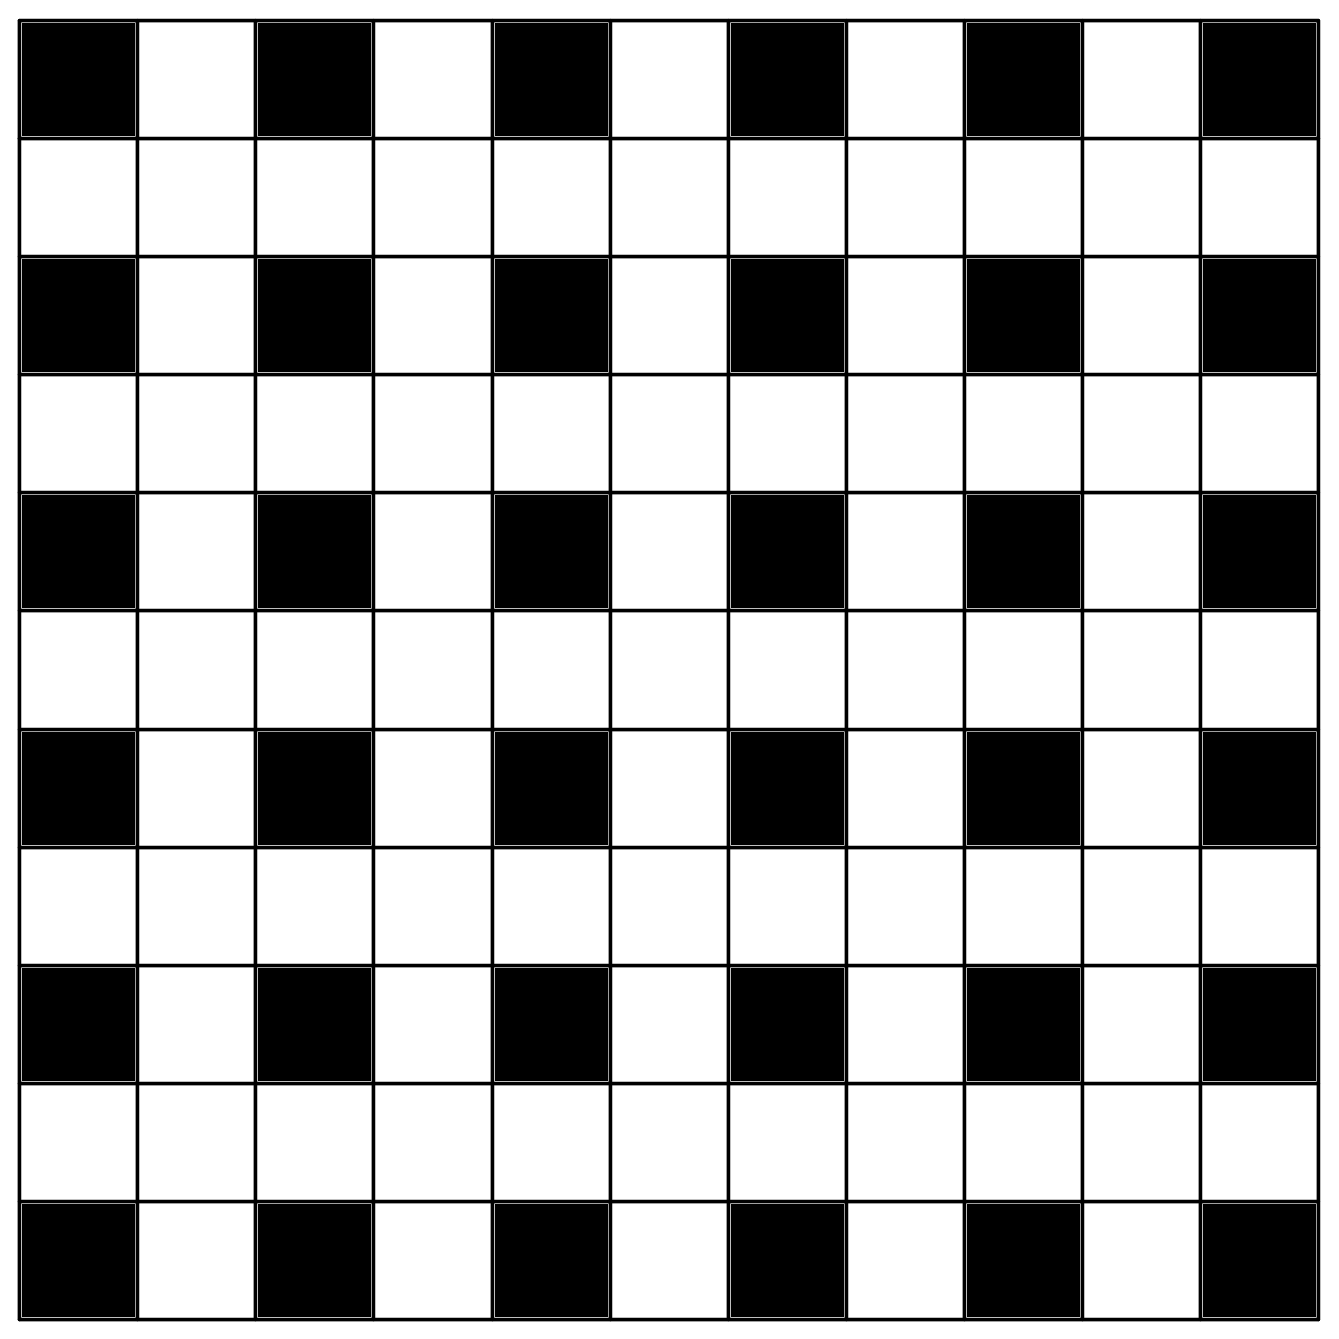
\includegraphics[width=5cm]{./aufgabe5-faerb.png}
\end{center}

Diese Färbung enthält $36$ schwarze Felder.
Wir stellen fest, dass jeder $2\times 2$-Block und jedes Skew-Tetromino genau ein  schwarzes Feld bedeckt. 

Wenn wir also genau $28,25,22,19,16$ respektive $13$ Blöcke der Fläche $4$ verwenden, dann verbleiben $8,11,14,17,20$ respektive $23$ schwarze Felder die mit $3,7,11,15,19$ respektive $23$ L-Triominos bedeckt werden müssten.

Wir stellen ebenfalls fest, dass ein L-Triomino höchstens $1$ schwarzes Feld bedecken kann. Wir brauchen also mindestens $23$ L-Triominos um das Brett zu bedecken.
Wie folgendes Bild zeigt, ist das auch tatsächlich möglich:

\begin{center}
  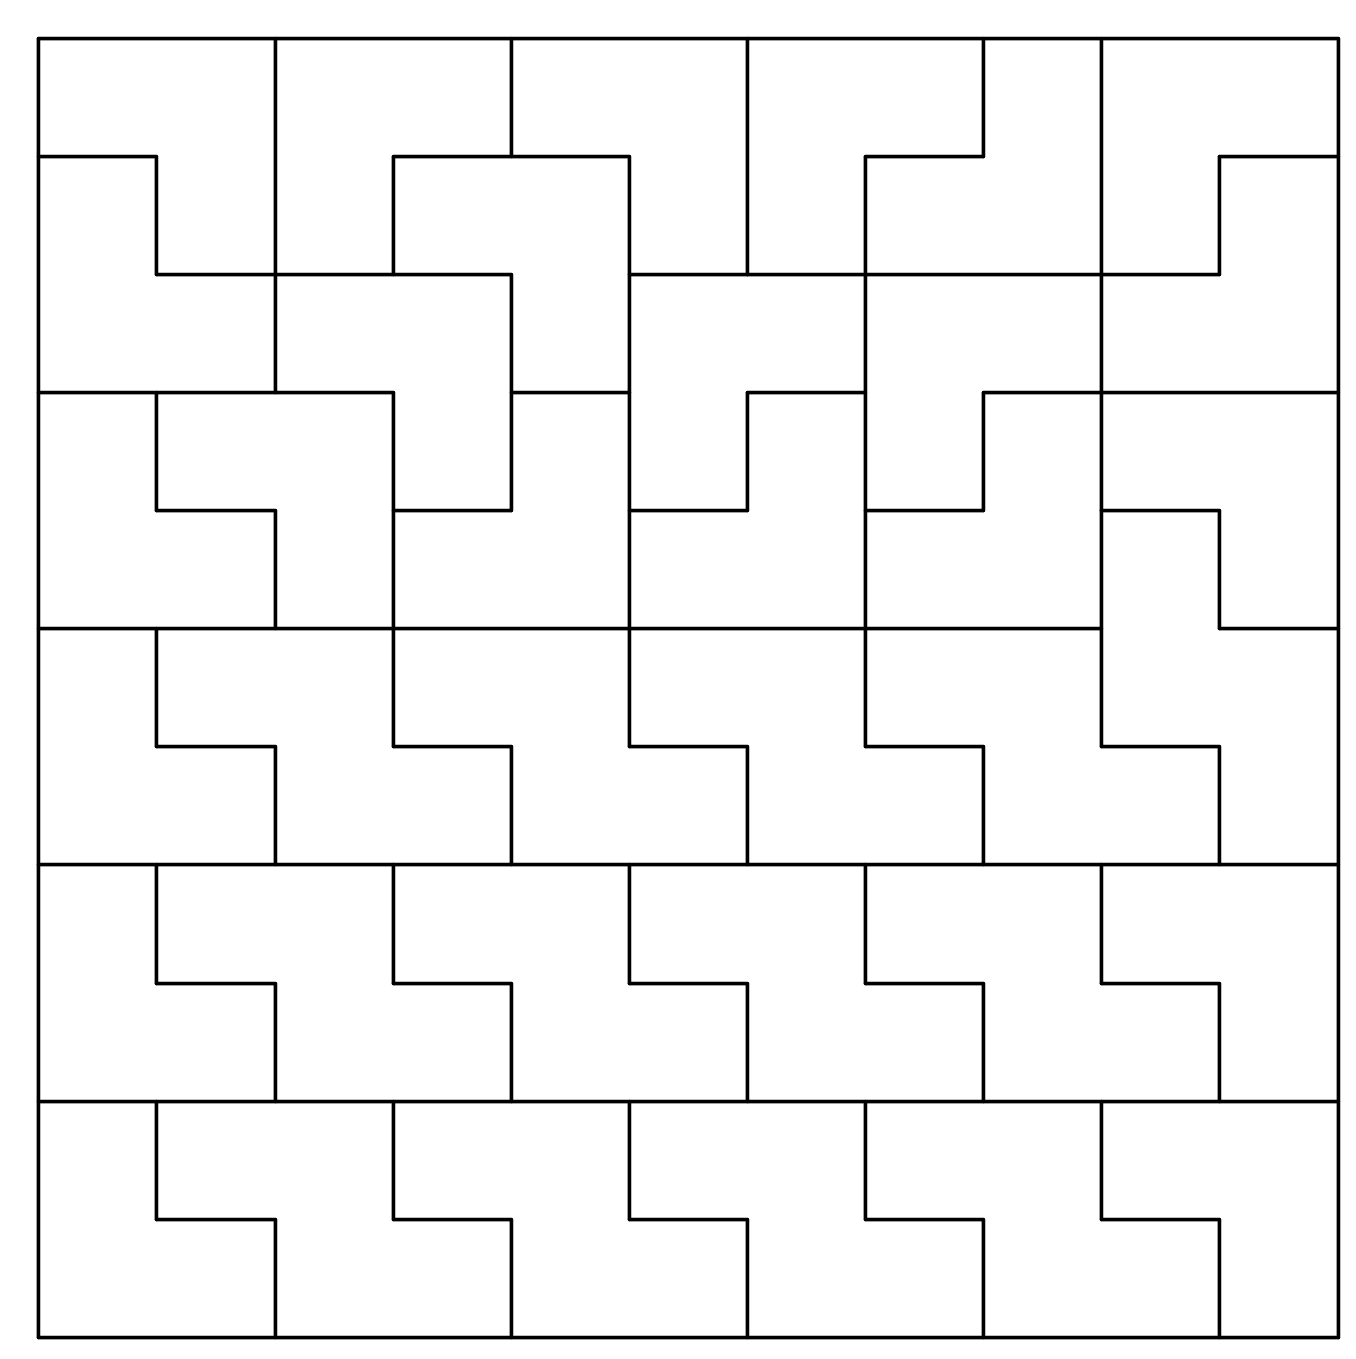
\includegraphics[width=5cm]{./aufgabe5-23.png}
\end{center}


\emph{Zum Punkteschema:} 
\begin{itemize}
  \item bla 1 Punkt
  \item blabla +1 Punkt
\end{itemize}
          



\end{enumerate}


\end{document}
